\documentclass[12pt]{letter}\usepackage[letterpaper,margin=0.65in]{geometry}\usepackage{textcomp}\usepackage{graphicx}\usepackage[rflt]{floatflt}\pagenumbering{gobble}\begin{document}\begin{floatingfigure}{0.15\textwidth}\raisebox{0pt}[0pt][0pt]{\raisebox{-2.5cm}{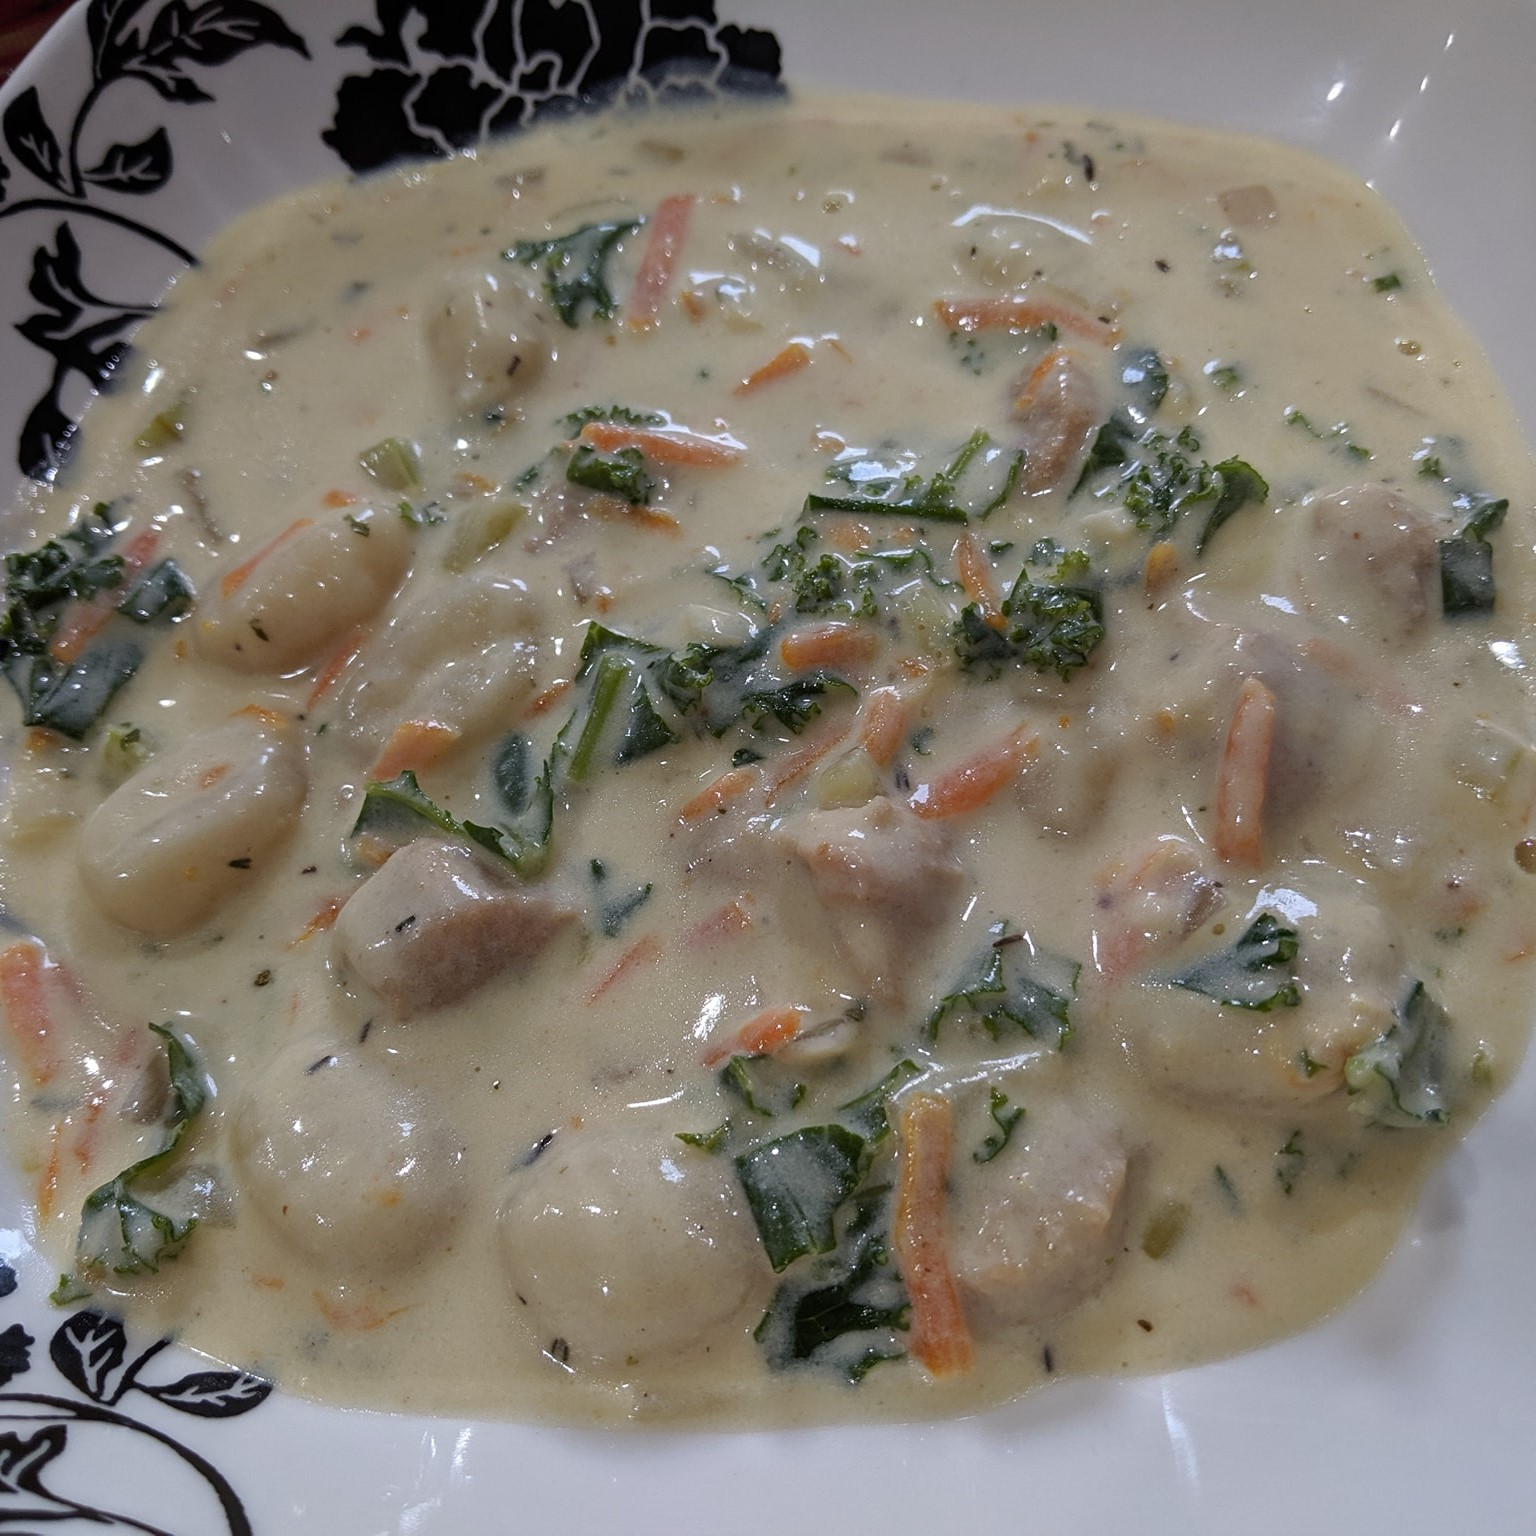
\includegraphics[width=0.15\textwidth]{creamy-gnocchi-soup}}}\end{floatingfigure}\begin{huge}Creamy Gnocchi Soup\end{huge}\newline\vspace{-2.5mm}\newline\renewcommand{\arraystretch}{1.1}\begin{tabular*}{\textwidth}{@{\extracolsep{\fill}}lr}A vegetarian version of an Olive Garden favorite\\Sunny C\end{tabular*}\newline\vspace{10mm}\newline\begin{huge}Ingredients\end{huge}\\\rule[2.8mm]{\textwidth}{.1pt}\vspace{-3mm}\begin{itemize}\item 4 cups vegetable broth, divided\item 1 qt half-and-half\item 16 oz ready-to-use gnocchi\item $\frac{3}{4}$ cup textured vegetable protein\item 2 cups kale, chopped\item 1 cup carrots, shredded\item 1 medium yellow onion, finely diced\item 2 stalks celery, finely diced\item 4 garlic cloves, minced\item $\frac{1}{2}$ teas dried thyme\item $\frac{1}{2}$ teas dried parsley flakes\item $\frac{1}{4}$ teas ground nutmeg\item 1 cube vegetable bouillon\item 4 tbs butter\item $\frac{1}{4}$ cup (30 grams) all-purpose flour\end{itemize}\vspace{7mm}\begin{huge}Directions\end{huge}\\\rule[2.8mm]{\textwidth}{.1pt}\vspace{-3mm}\begin{enumerate}\item Warm $\frac{3}{4}$ cup vegetable broth in small saucepan. Add textured vegetable protein and let sit until TVP is reconstituted.\item Melt butter in large stock pot. Sauté onion, celery, and garlic until onion is translucent.\item Add flour and cook for about 1 minute, whisking constantly.\item Slowly add half and half, whisking continuously until thickened, then repeat with vegetable broth.\item Add spices, whisking to combine, then add remaining ingredients and cook until carrots and kale are tender and gnocchi and veggie protein are warmed through.\end{enumerate}\end{document}